\documentclass[12pt]{standalone}

\usepackage{tikz}
    \usetikzlibrary{arrows.meta}
    
\usepackage{graphicx} % Работа с графикой \includegraphics{}
\graphicspath{{./pictures/}} % картинки в папке pictures

\usepackage{bm}
\newcommand{\bma}{{\bm{\alpha}}}
    
\begin{document}

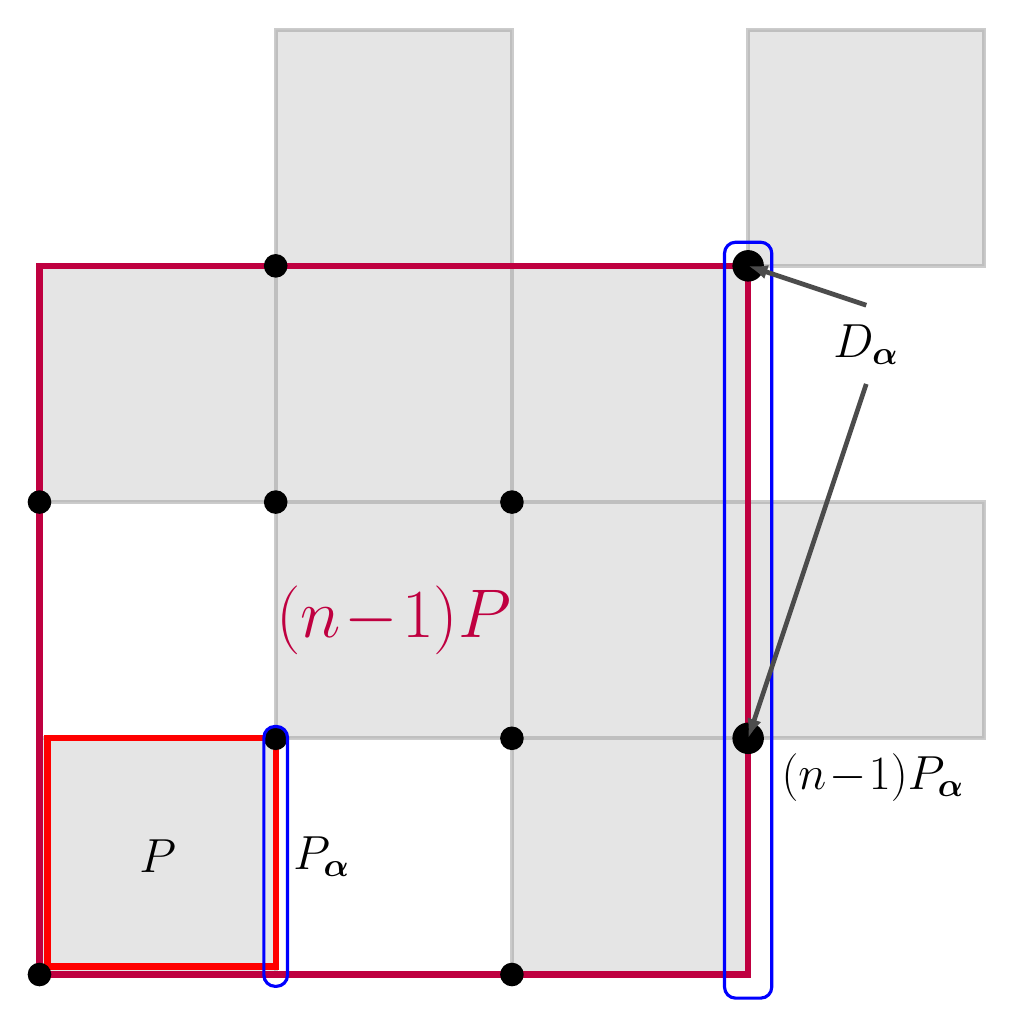
\begin{tikzpicture}
    % \draw[help lines] (0,0) grid (12,12);
    \draw[opacity=0.5,black!40,fill=black!20,line width=0.5mm]
        (0,0)rectangle(3,3) (6,0)rectangle(9,3)
        (3,3)rectangle(6,6) (6,3)rectangle(9,6)
        (9,3)rectangle(12,6) (0,6)rectangle(3,9)
        (3,6)rectangle(6,9) (6,6)rectangle(9,9)
        (3,9)rectangle(6,12) (9,9)rectangle(12,12);
    \draw[purple,line width=0.8mm] 
        (0,0)rectangle(9,9);
    \draw[red,line width=0.8mm] 
        (0.1,0.1)rectangle(3,3);
    % \node[shift={(1.5,1.5)}]
        % {\includegraphics[width=3cm]{frsq4.png}};
    \fill[black,line width=0.5mm]
        (0,0)circle(1.5mm) (6,0)circle(1.5mm)
        (3,3)circle(1.5mm) (6,3)circle(1.5mm)
        (9,3)circle(2mm) (0,6)circle(1.5mm)
        (3,6)circle(1.5mm) (6,6)circle(1.5mm)
        (3,9)circle(1.5mm) (9,9)circle(2mm);
    \draw[blue,line width=0.4mm,rounded corners]
        (8.7,-0.3)rectangle(9.3,9.3)
        (2.85,-0.15)rectangle(3.15,3.15);
    \node[shift={(1.5,1.5)}]{\LARGE$P$};
    % \draw[->,>={Latex[length=7pt]},blue!50,line width=0.6mm] (10.5,2)--(9.15,2);
    % \draw[->,>={Latex[length=7pt]},blue!50,line width=0.6mm] (4.5,2)--(3.15,2);
    \node[shift={(9.3,2.5)},right]{\LARGE$(n\!-\!1)P_\bma$};
    \node[shift={(3.1,1.5)},right]{\LARGE$P_\bma$};
    \node[shift={(10.5,8)}]{\LARGE$D_\bma$};
    \node[shift={(4.5,4.5)}, purple]{\Huge${(n\!-\!1)P}$};
    % \node[shift={(2,5)},above]{\LARGE$P$};
    % \node[shift={(3.7,1.5)},below]{\LARGE$\bma$};
    \draw[->,>={Latex[length=7pt]},black!70,line width=0.6mm] (10.5,7.5)--(9,3);
    \draw[->,>={Latex[length=7pt]},black!70,line width=0.6mm] (10.5,8.5)--(9,9);
    % \draw[->,>={Latex[length=7pt]},purple!70!black,line width=0.6mm] (4.5,10)--(4.5,9);
    % \draw[->,>={Latex[length=7pt]},red!50,line width=0.6mm] (2,5)--(2,3);
    % \draw[->,>={Latex[length=9pt]},line width=0.8mm] (1.5,1.5)--(4.5,1.5);
\end{tikzpicture}

\end{document}